\documentclass[conference]{IEEEtran}
\IEEEoverridecommandlockouts
\usepackage[utf8]{inputenc}
\usepackage[T1]{fontenc}
\usepackage{microtype}
\setlength{\emergencystretch}{1em}
\usepackage{amsmath,amssymb}
\usepackage{booktabs}
\usepackage{graphicx}
\usepackage{xcolor}
\usepackage{tikz}
\usepackage{cite}
\usepackage{balance}
\usepackage{xurl}
\usepackage[hidelinks]{hyperref}

\newcommand{\TEP}{TEP}
\newcommand{\PROTO}{\textsc{proto}}
\newcommand{\cond}[1]{\textsf{#1}}
\newcommand{\lu}{local-unseen}
\newcommand{\ls}{own-fault}

\begin{document}

\title{An LLM with Rule-Based Peer Insights\\
versus a Prototype Rule\\
for Fault Diagnosis under Extreme Label Skew}

\author{%
\IEEEauthorblockN{Luca Sorrentino\IEEEauthorrefmark{1},
Gabriele Piantadosi\IEEEauthorrefmark{2},
Antonio Galli\IEEEauthorrefmark{1},
Girolamo Di Francia\IEEEauthorrefmark{2} and
Carlo Sansone\IEEEauthorrefmark{1}}
\IEEEauthorblockA{\IEEEauthorrefmark{1}University of Naples Federico II,
Electrical Engineering and Information Technology Department, Napoli, 80125, Italy}
\IEEEauthorblockA{\IEEEauthorrefmark{2}ENEA CR-Portici,
Energy Technologies and Renewable Sources Department, Portici, 80055, Italy}
}

\maketitle

% ---------------------------------------------------------------------
\begin{abstract}
We study fault diagnosis when clients each hold normal data and examples of only one fault. In an offline Tennessee Eastman Process benchmark, a large language model (LLM) reads local examples and deterministic peer insights; a prototype rule and a FedAvg reference use the same development pool. The text exchange is inspired by Federation over Text but has no iterative client updates. A prospectively specified follow-up evaluates 256 new simulation runs (eight faults and Normal), seven language-model conditions and two numerical references. Adding the receiver's own-class summary to the peer-summary prompt raised own-fault accuracy by 20.8 percentage points (95\% CI 14.9--26.8; $p=4.65\times10^{-10}$). A content-free replacement for the peer block produced a similar own-fault gain despite using fewer prompt tokens. Neither comparison isolates the own-summary content effect, for which a matched control is absent. For F1 unseen in the receiver's local data, the peer-summary model exceeded a fixed-feature prototype rule by 86.3 points (Holm $p=1.91\times10^{-6}$); for F8 it fell 45.8 points below it (Holm $p=9.45\times10^{-4}$). FedAvg surpassed every primary-model prompt on pooled locally unseen faults, and both numerical references did so on Normal. A single server-side synthesis of all insights did not improve the primary model's observed accuracy over their unsynthesized form. A second configured LLM showed a similar own-fault gain, but its other comparisons were adverse or mixed and are exploratory. Peer summaries can support diagnosis without sharing raw client runs, yet gains depend on the fault, receiver role and output validity; this simulation establishes neither a privacy guarantee nor a deployed federated system.


\end{abstract}

\begin{IEEEkeywords}
federated learning, label distribution skew, large language models, in-context learning, fault diagnosis, Tennessee Eastman Process, multivariate time series
\end{IEEEkeywords}

% ---------------------------------------------------------------------
\section{Introduction}
\label{sec:intro}
Industrial sites may each have examples of their own faults but none of faults seen elsewhere. Can peer insights help a client diagnose those faults beyond its local examples, and how does that system compare with numerical references? Federated learning exchanges model updates without pooling raw client records~\cite{mcmahan2017fedavg}; severe label skew complicates that approach~\cite{li2022noniid}. Another option is to exchange compact diagnostic knowledge. Federation over Text (FoT) iteratively distills clients' language-model reasoning traces into a shared insight library~\cite{yao2026fot}. Here each client instead supplies one deterministic, rule-rendered summary of recurring observations, and the model reads these summaries once, in context. The setup is an offline test of that simpler exchange, not an implementation of FoT or an online federation protocol.

We compare a large language model (LLM) with local examples, peer summaries and optional own-class or synthesized summaries against a nearest-class-mean rule on fixed numerical features (\PROTO{}) and a fixed FedAvg reference. Development data are the separate data used to construct examples, summaries and numerical rules before evaluation. Eight Tennessee Eastman Process (\TEP{}) clients each hold Normal and one distinct fault. For a receiving client, a fault from another client is \emph{local-unseen}; a case of its own fault and a Normal case are separate outcomes. Every 5-hour case is evaluated for all eight receivers, but the physical simulation run, rather than the eight paired decisions, is the unit of inference.

An initial 96-run exploratory cohort suggested two follow-up questions. On 256 independent runs specified before generation, Family~A tests whether adding the own-class summary to the peer-summary prompt changes own-fault accuracy. Family~B revisits the opposing F1 and F8 local-unseen differences between the peer-summary LLM and \PROTO{}. Both fault classes remain in every all-fault summary. The seven-arm evaluation also measures Normal decisions, abstentions and malformed responses. A second LLM on the same grid supplies exploratory, configured-system comparisons under different serving controls. The central finding is a positive own-fault contrast alongside a strong adverse F8 contrast and a Normal advantage for the numerical references; neither a general text-over-number advantage nor an isolated semantic mechanism follows.

Our contribution is a run-paired, fixed-denominator comparison of text-sharing and numerical diagnostic configurations under class-disjoint fault ownership, with the negative and null results reported alongside gains. The study separates prespecified tests from descriptive follow-ups and records model abstentions and parsing failures. It measures simulated fault classification, not privacy, network performance or industrial deployment.


\section{Related Work}
\label{sec:related}

\paragraph{Parametric and prototype-based federation}
\mbox{FedAvg}~\cite{mcmahan2017fedavg} averages model parameters across clients. Li et al.~\cite{li2022noniid} find label skew the most challenging of the non-identically distributed (non-IID) settings they study; their hardest setting gives each client one label, whereas each of ours also holds Normal. FedProto~\cite{tan2022fedproto} forms class prototypes as means of learned embeddings; a server combines them to guide subsequent local training, and Tan et al. also describe nearest-prototype inference. In mechanical fault diagnosis, Fan et al.~\cite{fan2025prototype} study clients with a common Normal class and disjoint fault classes, using learned global prototypes to recognize locally unseen classes. Our prototype rule classifies by mean absolute (L1) distance to class means of fixed features, without representation learning or iterative optimization: a simple distributable rule, not a state-of-the-art federated baseline. We also evaluate FedAvg on the same clients and test cases: post hoc on the exploratory cohort and as one fixed reference in the follow-up (Section~\ref{sec:conditions}).

\paragraph{Textual federation and in-context collaboration}
FoT~\cite{yao2026fot} is the reference method: in each round, clients send reasoning traces to a server, which distills them into an insight library used by agents in context. Related approaches exchange natural-language compendia~\cite{wu2024fical}, iteratively refine answers~\cite{wang2025fedicl}, aggregate prompts optimized locally with textual gradients~\cite{chen2025fedtextgrad}, or study social learning between language models~\cite{mohtashami2023social}. Our peer insights are rendered once by a fixed rule-based procedure from recurring observations in each contributing client's development data. No LLM writes them, and in the peer-insight conditions there is no cross-client distillation, server-side merging or later revision. One follow-up condition, \cond{AGG}, adds a single server-side step in which the primary LLM synthesizes the eight insights into one library (Section~\ref{sec:conditions}). Server-side aggregation of client text is not new: FICAL concatenates client compendia~\cite{wu2024fical}, and FedTextGrad concatenates or summarizes client prompts over rounds~\cite{chen2025fedtextgrad}. \cond{AGG} is a single-cycle control inspired by FoT's server-side distillation, not FoT.

\paragraph{Trade-offs of shared knowledge}
In parametric federation, accuracy on a client's own data and on all clients' data are distinct objectives, and improving one can degrade the other~\cite{chen2022fedrod}. For LLMs, retrieved context can lower accuracy, even on questions answered correctly without it~\cite{mallen2023trust,yoran2024robust}. These precedents suggest that shared knowledge should not be judged on one outcome alone; we report the prespecified own-fault and Normal outcomes alongside local-unseen accuracy. Longer inputs can also affect LLM reasoning on otherwise identical tasks~\cite{levy2024same}, so we report prompt-token use (Section~\ref{sec:cost}) and treat length as a confound we cannot remove (Section~\ref{sec:limits}).

\paragraph{Time series, language and \TEP{} diagnosis}
Work linking time series and language includes structured program representations~\cite{kim2026t2sp} and signals-to-semantics zero-shot fault diagnosis (S2S-FDD)~\cite{li2025s2sfdd}. The \TEP{} simulator is a standard process-monitoring benchmark~\cite{downs1993tep,bathelt2015tep}. On \TEP{}, FaultExplainer~\cite{khan2025faultexplainer} gives an LLM principal component analysis (PCA)-based detection output and the top contributing variables; its unseen-fault scenario withholds a list of known root causes from the prompt, whereas \lu{} here means the receiving client has no local examples of the fault. S2S-FDD and FaultExplainer are centralized: no knowledge passes between clients. In simulated fault diagnosis, Lee et al.~\cite{lee2025agentic} report stronger LLM anomaly detection with summarized statistical inputs than with raw sensor readings, at best approaching a rule-based statistical baseline in $F_1$ score. Our rule-based procedure is deterministic and frozen; we make no claim about learned text representations.

We compare diagnosis by the primary LLM, using rule-based peer insights, against a prototype rule using fixed-feature class means, evaluating neither FoT nor FedProto as a complete algorithm.

% ---------------------------------------------------------------------
\section{Simulated Setting and Compared Systems}
\label{sec:method}

Figure~\ref{fig:method-flow} shows the text and prototype paths; the FedAvg reference uses the same numerical signatures. The following subsections define the offline construction and decision-time inputs.

% Method overview (TikZ, one column, basic TikZ only). Both panels read top to bottom.
% Arrows = derivation and use of stored artifacts, not communication; dashed = peer insights (some conditions only).


\begin{figure}[t]
\centering
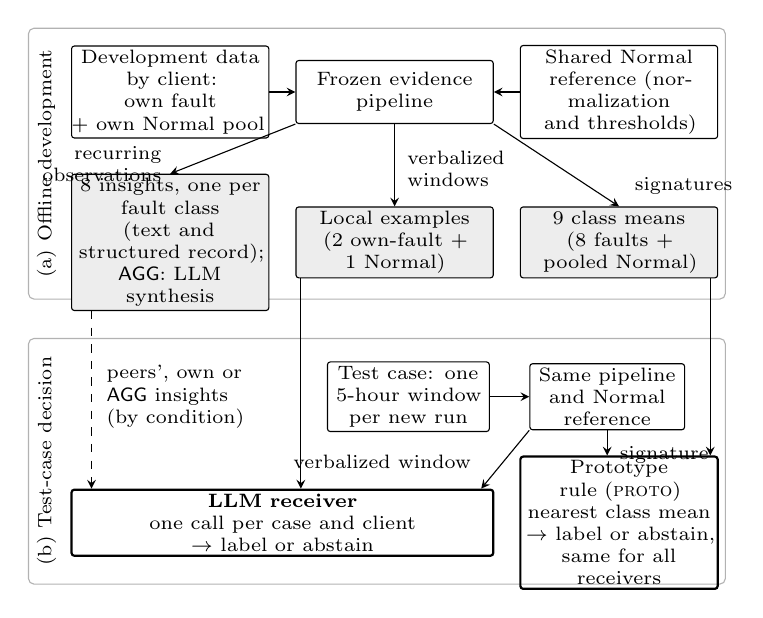
\begin{tikzpicture}[x=1mm,y=1mm,>=stealth,
  box/.style={draw,rounded corners=1pt,align=center,font=\scriptsize,inner sep=1.5pt,text width=24mm,minimum height=8mm},
  art/.style={box,fill=gray!14},
  sys/.style={box,thick},
  lab/.style={font=\scriptsize,inner sep=1pt,align=left}]
% panel frames and side titles
\draw[gray!60,rounded corners=2pt] (0,-24.8) rectangle (88.5,9.6);
\draw[gray!60,rounded corners=2pt] (0,-61) rectangle (88.5,-29.8);
\node[font=\scriptsize,rotate=90] at (2.3,-7.6) {(a) Offline development};
\node[font=\scriptsize,rotate=90] at (2.3,-45.4) {(b) Test-case decision};
% (a) data and pipeline
\node[box] (cli) at (18,1.5) {Development data\\by client: own fault\\+ own Normal pool};
\node[box] (pipe) at (46.5,1.5) {Frozen evidence\\pipeline};
\node[box] (ref) at (75,1.5) {Shared Normal\\reference (normalization\\and thresholds)};
\draw[->] (cli) -- (pipe);
\draw[->] (ref) -- (pipe);
% (a) stored artifacts
\node[art] (ins) at (18,-17.6) {8 insights, one per\\fault class (text and\\structured record);\\\cond{AGG}: LLM synthesis};
\node[art] (loc) at (46.5,-17.6) {Local examples\\(2 own-fault +\\1 Normal)};
\node[art] (mean) at (75,-17.6) {9 class means\\(8 faults +\\pooled Normal)};
\draw[->] (pipe.south west) -- (ins.north);
\draw[->] (pipe.south) -- (loc.north);
\draw[->] (pipe.south east) -- (mean.north);
\node[lab,anchor=east,align=right] at (17.3,-7.6) {recurring\\observations};
\node[lab,anchor=west] at (47.7,-8.2) {verbalized\\windows};
\node[lab,anchor=west] at (76.6,-10.4) {signatures};
% (b) test case and pipeline
\node[box,text width=19.5mm] (win) at (48.25,-37.2) {Test case: one\\5-hour window\\per new run};
\node[box,text width=18.6mm] (pipe2) at (73.5,-37.2) {Same pipeline\\and Normal\\reference};
\draw[->] (win) -- (pipe2);
% (b) the two systems
\node[sys,text width=52.5mm] (llm) at (32.25,-53.2)
  {\textbf{LLM receiver}\\one call per case and client\\$\rightarrow$ label or abstain};
\node[sys] (proto) at (75,-53.2)
  {Prototype rule (\PROTO{})\\nearest class mean\\$\rightarrow$ label or abstain,\\same for all receivers};
% stored artifacts used at decision time
\draw[->,dashed] (8,0 |- ins.south) -- (8,0 |- llm.north);
\draw[->] (34.6,0 |- loc.south) -- (34.6,0 |- llm.north);
\draw[->] (86.6,0 |- mean.south) -- (86.6,0 |- proto.north);
\node[lab,anchor=west] at (9.5,-37.2) {peers', own or\\\cond{AGG} insights\\(by condition)};


% test case to the two systems
\draw[->] (pipe2.south west) -- (57.5,0 |- llm.north);
\node[lab,anchor=east] at (56.6,-45.4) {verbalized window};
\draw[->] (pipe2.south) -- (pipe2.south |- proto.north);
\node[lab,anchor=west] at (74.7,-44.6) {signature};
\end{tikzpicture}
\caption{Offline development and test-case decision paths. Arrows denote derivation and use of stored artifacts, not communication between clients.}
\label{fig:method-flow}
\end{figure}

\subsection{Clients, labels and units of analysis}
Eight simulated clients observe the same \TEP{} plant, each owning one fault class: three step changes (F1--F3), two random variations (F8, F10), one slow drift (F13) and two sticking valves (F14, F15)~\cite{downs1993tep}. The development pool is partitioned by client: each has labeled development data for its own fault and its own Normal pool of 40 windows from five runs. The shared Normal reference consists of separate development Normal data, distinct from the clients' Normal pools; it is not private client training data, but its use departs from strict federation (Section~\ref{sec:limits}). The label space is $\{F1,F2,F3,F8,F10,F13,F14,F15,\text{Normal}\}$; a system outputs one label or abstains.

A \emph{case} is a 5-hour window from one run. Each case is paired with all eight clients, the receivers in the LLM conditions. A fault case yields one \emph{own-fault} pair with the client that owns its true fault class and seven \emph{\lu} pairs with the other clients; a Normal case yields eight \emph{Normal} pairs. This offline setup runs no federated communication protocol.

\subsection{Shared evidence pipeline}
The LLM and numerical references use one frozen evidence pipeline. Each 5-hour window has 300 one-minute samples for each of 41 measured variables (XMEAS). For each variable, the pipeline computes four statistics (mean shift (``level shift'' in the generated text), slope (linear trend), residual variability (standard deviation after linear detrending) and sample-to-sample variation (standard deviation of successive differences)), normalized using the shared Normal reference, and compares each with a fixed threshold calibrated on the same reference. Rapid variability is flagged only when both the residual and sample-to-sample statistics exceed their thresholds; an overall dispersion ratio is computed separately.

For the LLM, the pipeline renders each sensor window from a simulated run as a \emph{verbalized window}, a rule-generated English textual description of the window. It names the leading variable (the largest above-threshold magnitude) for each statistic (or says none), adds the leading variable for rapid variability when present and reports the largest dispersion ratio (window standard deviation divided by reference standard deviation). From the same evidence, the pipeline builds a 697-component numerical signature (feature vector) for the prototype rule, with 17 fields per variable: four each for mean shift and slope (active fraction, sign balance, late-active fraction and longest same-sign run) and three each for residual variability, sample-to-sample variation and rapid variability (active fraction, late-active fraction and longest run). For a single window, these fields record which thresholds fired and their signs, not magnitudes. The signature spans all variables but excludes the dispersion ratio, so the two summaries of the case differ.

The test case's verbalized window includes the absolute observed interval (hours) as fixed-onset context (faults begin at hour 25), but no fault label, run or stream ID, or file name. The interval does not identify the fault; local examples and any peer insights are labeled.

\subsection{Peer insights from recurring observations}
For each fault class, 40 development windows from five runs are scanned over three time spans (25--65, 25--35 and 35--65~h) for candidate observations. Candidates name the most frequent leading variable for mean shift, slope, residual variability, sample-to-sample variation or overall dispersion, or note no threshold exceedances. A candidate is retained as a recurring observation if it holds in at least half the windows of its span. A shorter-span candidate is nevertheless discarded when it repeats the variable, or the all-quiet observation, of a retained full-span candidate of the same kind; 30 of 144 were retained. Each retained observation also reports its frequency in the contributing client's Normal development windows for that span. F3 and F15 produced only an all-quiet observation, which also describes most Normal windows.

A fixed rule-based procedure renders the retained observations as one insight per fault class in two forms: natural-language text and a structured record. Both keep a class-bearing ID and name the class. A parse-back check confirms that both renderings contain the same 30 observations and headers, but does not show that an LLM uses them in the same way.

An excerpt from the actual \texttt{P05-INS-F1} insight, in natural language: ``Between 25 and 65 h, the largest above-threshold level shift is on XMEAS-1 in 40 of 40 development windows of F1 (positive in 40, negative in 0).'' The structured record includes \texttt{"observation": "largest above-threshold level shift"}, \texttt{"variable": "XMEAS-1"}, \texttt{"class\_windows": 40}, \texttt{"positive": 40} and \texttt{"negative": 0}. Both full renderings also note that this occurs in 0 of 40 Normal development windows of the contributing client; other F1 observations and fields are omitted.

\subsection{Conditions and prototype rule}
\label{sec:conditions}
All LLM conditions use the same open-weight LLM, the primary LLM (\texttt{qwen3.5-122b}), on a local endpoint, with a shared system prompt, the receiver's local block, the test case's verbalized window and strict four-field JSON output (\texttt{predicted\_label}, \texttt{abstain}, \texttt{used\_insight\_ids}, \texttt{reasoning\_summary}). Each receiver's fixed local block holds three local examples (in-context demonstrations): two verbalized windows of its own fault and one from its own Normal pool, at window positions fixed before any content was inspected. Generation uses temperature 0 and a fixed seed, with a 1,024-token thinking budget and up to 2,048 completion tokens. Conditions vary in the insight block that follows the local block (for peer insights, the seven in fixed fault-number order):
\begin{itemize}[\IEEEsetlabelwidth{\cond{FULL}}]
\item[\cond{A0}] no peer insights (local-only);
\item[\cond{B0}] seven peers' natural-language insights;
\item[\cond{S0}] structured records encoding the same seven peer insights as \cond{B0};
\item[\cond{SELF}] \cond{A0} plus the receiver's own-class insight in natural language;
\item[\cond{FULL}] \cond{B0} plus the same own-class insight, so that the receiver reads all eight insights;
\item[\cond{AGG}] in place of the insights, one library that the primary LLM synthesized from the eight insights;
\item[\cond{PL0}] \cond{B0} with its peer block replaced by generic process-monitoring text of the same byte length, but not the same token count (placebo).
\end{itemize}
\cond{S0} encodes the same seven peer insights as \cond{B0} in a structured rendering; it ran later and produces longer prompts, so their comparison does not isolate format. \cond{A0}, \cond{B0}, \cond{SELF} and \cond{FULL} cross peer-insight presence with own-insight presence ($2\times2$).

The \cond{AGG} library was written once, before any test use, from the eight natural-language insights alone: in two requests the primary LLM listed relations between insights and wrote 13 entries, eight on single classes and five contrasting two classes. After one permitted correction cycle it was accepted on a source audit, not on diagnostic accuracy.

The prototype rule, denoted \PROTO{}, is a non-LLM rule fixed on development data, using class means computed from development signatures: 40 windows for each of eight faults and 320 pooled Normal windows. For each case, \PROTO{} selects the class with minimum mean absolute distance over 697 components, abstaining if another class is within $10^{-12}$ of the minimum. It outputs one receiver-independent prediction per case, copied across receiver pairs for paired evaluation.

The LLM and \PROTO{} receive different inputs, and the LLM receiver gets no separate Normal insight: it sees one local Normal example, whereas \PROTO{} uses the mean of 320 Normal windows. This asymmetry matters when interpreting false alarms. We compare complete systems with unequal decision-time information.

The follow-up adds one numerical reference fixed in advance: logistic regression on the 697-component signatures, trained with FedAvg on the eight clients' development data (50 rounds, five local epochs per round, learning rate 0.3, no regularization, five seeds, class probabilities averaged). Its settings were chosen by cross-validation on development data, but this recipe was named as the reference only after its exploratory-cohort results were known. Like \PROTO{}, it predicts once per case. The parameters used are not those behind the exploratory-cohort results: they were rebuilt from development data alone and frozen before any follow-up case was scored (Section~\ref{sec:limits}).

A separately scheduled, non-blocking supplementary track applies all seven conditions to a second open-weight LLM, \texttt{gpt-oss-120b}, on the same cases. It uses temperature 0, seed 20260927, top-$p$ 1, unrestricted top-$k$, low reasoning effort, a 4,096-token output cap and a 16,384-token context; requests run at concurrency four. The primary endpoint reports vLLM 0.27.1, as does this supplementary service, but model weights, request envelope and generation controls differ. Thus cross-model comparisons describe configured systems (Section~\ref{sec:limits}).

\subsection{Reused development components}
\label{sec:provenance}
Reused development components have pinned source hashes: the qualified Simulink model with Philox-controlled fault injection; frozen features, thresholds and verbalization, with current English wording; labels and fault ownership; the 80-run development pool; and the shared Normal reference. \PROTO{} matches its source rule and development outputs. Earlier evaluation runs, predictions and results are not pooled into either evaluation cohort. The follow-up reuses these components; from the exploratory cohort it takes only the choice of hypotheses, conditions and FedAvg reference (Section~\ref{sec:protocol}).

% ---------------------------------------------------------------------
\section{Evaluation Design}
\label{sec:protocol}
\subsection{Cohorts and window selection}
The shared development pool contains 80 runs and a separate shared Normal reference; development components and the rule for selecting one post-onset 5-hour window per run were fixed before either evaluation cohort. The earlier exploratory cohort has 96 runs (eight per fault, 32 Normal). Its three prespecified local-unseen contrasts were analyzed before follow-up planning and are presented only as exploratory context. The follow-up comprises 256 new runs, 24 per fault and 64 Normal, generated on disjoint random-number streams. Each run lasts 65 hours, with fault onset at hour 25. Eight half-open 5-hour windows cover $[25,65)$~h. For class position $k$ and class offset $o_c$, the selected ordinal is $j=1+((k-1+o_c)\bmod 8)$, giving interval $[25+5(j-1),30+5(j-1))$. Offsets are 0--7 in the listed fault order and 0 for Normal. Every fault covers each window three times; Normal covers each eight times. All 256 primary runs passed the technical checks, with no replacement. The cohorts are not pooled. This produces 192 own-fault, 1,344 local-unseen and 512 Normal receiver pairs per arm. The seven LLM arms (\cond{A0}, \cond{B0}, \cond{FULL}, \cond{SELF}, \cond{AGG}, \cond{S0}, \cond{PL0}) received 14,336 requests in total. \cond{A0}/\cond{B0}, \cond{FULL}/\cond{SELF}, and \cond{AGG} ran in successive interleaved tiers; \cond{S0}/\cond{PL0} ran later. The second LLM used the same case grid but different generation and serving controls.

\subsection{Outcomes and run-level inference}
The endpoint is exact-label correctness at the fixed planned denominator, with no top-$k$ or alias credit. Wrong-fault labels, faults missed as Normal, and false alarms on Normal are distinct from non-answers. A false own-label assignment means predicting the receiving client's fault when the true class differs. One response is scored per planned key, without voting or content-based retries. Abstained, parser-rejected, truncated and missing responses count as non-correct and are reported separately; an HTTP 200 response is not a correct diagnosis. Let $Y_{a,r,c}$ be one for a valid exact-label answer by arm $a$ on run $r$ and receiver $c$, and zero otherwise. For a contrast $a-b$ and receiver set $C_r$,
\begin{equation}
d_r=\frac{1}{|C_r|}\sum_{c\in C_r}(Y_{a,r,c}-Y_{b,r,c}),\qquad
\widehat\Delta=\frac{1}{K}\sum_{f=1}^{K}\bar d_f.
\end{equation}
The set contains one owner for own-fault, seven non-owners for local-unseen, or eight receivers for Normal. Fault contrasts weight the $K$ included classes equally; each $\bar d_f$ averages physical runs within class. Normal instead averages its 64 run differences. For Family~A, $K=8$, $n_f=24$, and
\begin{equation}
\widehat{\mathrm{SE}}^2=\frac{1}{K^2}\sum_f v_f,\quad
v_f=\frac{s_f^2}{n_f},\quad
\nu=\frac{(\sum_f v_f)^2}{\sum_f v_f^2/(n_f-1)},
\end{equation}
where $s_f^2$ is the sample variance of the run differences. Receiver rows and development windows from one run are not independent replications. Family~A is \cond{FULL}$-$\cond{B0} on the 192 own-fault runs, tested with a class-stratified $t$ statistic and Welch--Satterthwaite degrees of freedom~\cite{welch1947,satterthwaite1946}. Family~B tests \cond{B0}$-$\PROTO{} on the seven local-unseen receivers of each F1 or F8 run, using all $2^{24}$ whole-run sign assignments, including ties in the two-sided tail, and Holm adjustment across those two tests~\cite{holm1979}. Each family has its own two-sided $\alpha=0.05$; no joint 0.05 claim is made. The three prespecified descriptive partitions are all eight faults, the six excluding F1/F8, and F1/F8 alone. Other arm comparisons are descriptive too. Pointwise percentile intervals use 20,000 within-fault run resamples, carrying all arms and receivers together; Normal resamples its whole runs. Qwen uses PCG64 seed 20261006 and the supplementary track seed 20261007. These are run-level, not receiver-level, resamples~\cite{field2007bootstrap}. The planned descriptive contrasts are \cond{B0}$-$\cond{A0}, \cond{SELF}$-$\cond{A0}, \cond{FULL}$-$\cond{SELF}, their $2\times2$ interaction, \cond{AGG}$-$\cond{FULL}, \cond{S0}$-$\cond{B0}, \cond{PL0}$-$\cond{B0}, and \cond{B0} against both numerical references. No equivalence margin was set. A dated local specification fixed the Qwen follow-up analyses before generation and outcome opening; the exploratory cohort had already motivated the hypotheses. The gpt-oss analysis was fixed after primary-model requests began and is therefore exploratory descriptive even though it uses the same new cases. Its execution could neither delay nor alter the Qwen analysis or its outcome-opening decision. Qwen truth was first joined on 7 October 2026 after the reviewed technical opening decision; no outcome-based case replacement followed.


\section{Results}
\label{sec:results}
\subsection{Follow-up coverage and primary contrasts}
All 14,336 Qwen requests received an HTTP 200 terminal response on one attempt, but only 11,912 met the operational answer contract; 2,343 abstained, 43 were rejected by an extra client-side 1,200-character summary cap despite satisfying the transmitted JSON schema, and 38 were truncated. These outcomes remain in the denominators. Gpt-oss likewise completed 14,336 requests, with 11,908 valid and 2,428 abstentions. Table~\ref{tab:t2main} shows the prespecified Qwen tests and principal descriptive comparisons; Table~\ref{tab:t2arms} reports every Qwen arm and the numerical references. Local-unseen \cond{SELF} and \cond{PL0} accuracy is near zero chiefly because the arms abstain on 889 and 473 of 1,344 keys, respectively.

\begin{table*}[t]
\centering\footnotesize
\caption{New 256-run follow-up. Correctness and contrasts are percentage points (pp) at the fixed denominator. Family A uses 192 own-fault physical runs; Family B uses 24 runs per fault, averaging seven locally unseen receivers within run. The gpt-oss rows are exploratory descriptive, not additional tests.}
\label{tab:t2main}
\setlength{\tabcolsep}{4pt}
\begin{tabular}{llrrl}
\toprule
Configured system / contrast & Outcome & Difference (pp) & Accuracies (\%) & Interval or test \\
\midrule
Qwen \cond{FULL}$-$\cond{B0} & Own fault & $+20.833$ & 90.104 / 69.271 & 95\% CI $[+14.875,+26.792]$; $p=4.649\times10^{-10}$ \\
Qwen \cond{B0}$-$\PROTO{}, F1 & Local-unseen & $+86.310$ & 98.810 / 12.500 & Holm $p=1.907\times10^{-6}$ \\
Qwen \cond{B0}$-$\PROTO{}, F8 & Local-unseen & $-45.833$ & 37.500 / 83.333 & Holm $p=9.450\times10^{-4}$ \\
Qwen \cond{B0}$-$\PROTO{}, all faults & Local-unseen & $+3.720$ & 64.658 / 60.938 & Descriptive pointwise 95\% $[+0.074,+7.366]$ \\
Gpt-oss \cond{FULL}$-$\cond{B0} & Own fault & $+22.917$ & 61.979 / 39.062 & Descriptive pointwise 95\% $[+16.667,+29.167]$ \\
Gpt-oss \cond{B0}$-$\PROTO{} & Local-unseen & $-9.524$ & 51.414 / 60.938 & Descriptive pointwise 95\% $[-13.616,-5.357]$ \\
\bottomrule
\end{tabular}

\end{table*}

\begin{table*}[t]
\centering\footnotesize
\caption{Follow-up Qwen operational accuracy by receiver role and terminal response state, all at planned denominators (2,048 pairs per LLM arm). Abstentions, parser rejections and truncations are retained as non-correct. Numerical rules issue one receiver-independent prediction per case and have no LLM response states.}
\label{tab:t2arms}
\setlength{\tabcolsep}{5pt}
\begin{tabular}{lrrrrrrr}
\toprule
Arm & Own (\%) & Local-unseen (\%) & Normal (\%) & Valid & Abstain & Rejected & Truncated \\
\midrule
\cond{A0} & 85.4 & 5.1 & 78.1 & 1747 & 252 & 21 & 28 \\
\cond{B0} & 69.3 & 64.7 & 72.3 & 1938 & 106 & 3 & 1 \\
\cond{FULL} & 90.1 & 62.2 & 70.5 & 1934 & 105 & 4 & 5 \\
\cond{SELF} & 82.3 & 0.1 & 72.7 & 1021 & 1024 & 2 & 1 \\
\cond{AGG} & 87.5 & 62.2 & 64.6 & 1841 & 200 & 5 & 2 \\
\cond{S0} & 69.3 & 62.6 & 69.7 & 1920 & 125 & 3 & 0 \\
\cond{PL0} & 89.6 & 2.7 & 74.8 & 1511 & 531 & 5 & 1 \\
\PROTO{} & 60.9 & 60.9 & 96.9 & -- & -- & -- & -- \\
FedAvg & 72.9 & 72.9 & 100.0 & -- & -- & -- & -- \\
\bottomrule
\end{tabular}

\end{table*}

Table~\ref{tab:faults} decomposes the own-fault contrast by fault and run gains/losses. The primary Qwen Family~A estimate is $+20.833$~pp (95\% CI $[+14.875,+26.792]$, $p=4.649\times10^{-10}$): 45 own-fault runs gained, five lost and 142 tied. F1 ($+62.5$~pp), F3 ($+45.8$), F8 ($+33.3$) and F15 ($+20.8$) carry most of the mean. F2 and F10 are unchanged at ceiling, F13 has one gain and one loss, and four F15 runs are worse under \cond{FULL}. Three of these 192 runs share a model-facing input with another run; the prespecified point-only drop sensitivity changes the estimate to $+20.901$~pp on 189 runs, without recomputing a test. The own-class summary therefore improves this complete Qwen prompt configuration on average, but there is no matched generic block in place of the own-class summary to identify its content contribution: \cond{PL0}$-$\cond{B0} reaches $+20.313$~pp on the same outcome despite using content-free byte-matched peer text, with a later serving window. Own-fault \cond{B0}$-$\cond{A0} is $-16.146$~pp. Without peers, the complementary own-summary effect \cond{SELF}$-$\cond{A0} is $-3.125$~pp; the descriptive $2\times2$ interaction is $+23.958$~pp. PL0 replaces peer content, not own-class content; it is therefore not a direct placebo for the added own-class summary. These descriptive controls couple content, length, format and possibly serving time.

\begin{table}[t]
\centering\footnotesize
\caption{Qwen fault-level follow-up. The own-fault column is the paired \cond{FULL}$-$\cond{B0} difference (24 runs/fault); local-unseen columns are fixed-denominator accuracy across seven receivers (168 pairs/fault). These rows are descriptive except the separately tested F1 and F8 contrasts in Table~\ref{tab:t2main}.}
\label{tab:faults}
\setlength{\tabcolsep}{2.5pt}
\begin{tabular}{lrrrrrr}
\toprule
Fault & Own $\Delta$ (pp) & Gain & Loss & Tie & Local B0 (\%) & Local \PROTO{} (\%) \\
\midrule
F1 & $+62.5$ & 15 & 0 & 9 & 98.8 & 12.5 \\
F2 & $+0.0$ & 0 & 0 & 24 & 100.0 & 100.0 \\
F3 & $+45.8$ & 11 & 0 & 13 & 1.8 & 4.2 \\
F8 & $+33.3$ & 8 & 0 & 16 & 37.5 & 83.3 \\
F10 & $+0.0$ & 0 & 0 & 24 & 100.0 & 100.0 \\
F13 & $+0.0$ & 1 & 1 & 22 & 72.6 & 87.5 \\
F14 & $+4.2$ & 1 & 0 & 23 & 100.0 & 100.0 \\
F15 & $+20.8$ & 9 & 4 & 11 & 6.5 & 0.0 \\
\bottomrule
\end{tabular}

\end{table}

\begin{table*}[t]
\centering\footnotesize
\caption{Follow-up fixed-denominator accuracy by fault for every Qwen arm and both numerical references. Each own-fault value has 24 physical runs; each local-unseen value has the same 24 runs evaluated for seven receivers. These are descriptive rates, not additional fault-level tests.}
\label{tab:allfaults}
\setlength{\tabcolsep}{6.5pt}
\begin{tabular}{lrrrrrrrrr}
\toprule
Fault & A0 & B0 & FULL & SELF & AGG & S0 & PL0 & \PROTO{} & FedAvg \\
\midrule
\multicolumn{10}{l}{\emph{Own-fault accuracy (\%)}} \\
F1 & 91.7 & 33.3 & 95.8 & 100.0 & 100.0 & 70.8 & 100.0 & 12.5 & 100.0 \\
F2 & 95.8 & 100.0 & 100.0 & 100.0 & 100.0 & 100.0 & 100.0 & 100.0 & 100.0 \\
F3 & 75.0 & 33.3 & 79.2 & 45.8 & 83.3 & 29.2 & 70.8 & 4.2 & 0.0 \\
F8 & 91.7 & 58.3 & 91.7 & 100.0 & 79.2 & 70.8 & 100.0 & 83.3 & 83.3 \\
F10 & 100.0 & 100.0 & 100.0 & 100.0 & 100.0 & 100.0 & 100.0 & 100.0 & 100.0 \\
F13 & 95.8 & 75.0 & 75.0 & 91.7 & 75.0 & 75.0 & 100.0 & 87.5 & 100.0 \\
F14 & 100.0 & 95.8 & 100.0 & 100.0 & 100.0 & 100.0 & 100.0 & 100.0 & 100.0 \\
F15 & 33.3 & 58.3 & 79.2 & 20.8 & 62.5 & 8.3 & 45.8 & 0.0 & 0.0 \\
\midrule
\multicolumn{10}{l}{\emph{Local-unseen accuracy (\%)}} \\
F1 & 31.0 & 98.8 & 97.6 & 0.6 & 95.2 & 96.4 & 14.3 & 12.5 & 100.0 \\
F2 & 0.0 & 100.0 & 100.0 & 0.0 & 99.4 & 100.0 & 0.0 & 100.0 & 100.0 \\
F3 & 0.0 & 1.8 & 1.8 & 0.0 & 6.5 & 4.8 & 0.0 & 4.2 & 0.0 \\
F8 & 0.0 & 37.5 & 26.2 & 0.0 & 31.5 & 22.0 & 0.0 & 83.3 & 83.3 \\
F10 & 8.3 & 100.0 & 100.0 & 0.6 & 100.0 & 100.0 & 4.8 & 100.0 & 100.0 \\
F13 & 0.0 & 72.6 & 72.0 & 0.0 & 64.9 & 72.0 & 0.6 & 87.5 & 100.0 \\
F14 & 1.2 & 100.0 & 99.4 & 0.0 & 100.0 & 100.0 & 1.8 & 100.0 & 100.0 \\
F15 & 0.6 & 6.5 & 0.6 & 0.0 & 0.0 & 6.0 & 0.0 & 0.0 & 0.0 \\
\bottomrule
\end{tabular}

\end{table*}

Family~B rejects in opposite directions. On F1 local-unseen decisions, Qwen \cond{B0} exceeds \PROTO{} by $+86.310$~pp (Holm $p=1.907\times10^{-6}$); on F8 it falls below by $-45.833$~pp (Holm $p=9.450\times10^{-4}$). The latter is an adverse result for the LLM. F1's 24 physical runs contain one duplicate model-facing input pair (23 distinct inputs); dropping one member yields a point-only estimate of $+85.714$~pp, without a new test. Pooled across all eight faults, Qwen \cond{B0}$-$\PROTO{} is only $+3.720$~pp with a descriptive pointwise interval $[+0.074,+7.366]$; without F1/F8 it is $-1.786$~pp $[-4.365,+0.397]$. The all-fault pointwise interval is not a third rejection. F3 and F15 local-unseen scores remain near floor across systems (Table~\ref{tab:allfaults}). FedAvg also exceeds every Qwen arm on pooled local-unseen accuracy (72.917\% versus at most 64.658\%); \cond{B0}$-$FedAvg is $-8.259$~pp. Two numerical references exceed every Qwen prompt on Normal: \PROTO{} scores 96.875\%, FedAvg 100\%, and the seven Qwen arms 64.648--78.125\%. The comparator-specific numerical margin ranges from 18.750 to 35.352~pp.

Table~\ref{tab:supplement} gives all supplementary arms. The gpt-oss track also has a positive within-system own-fault \cond{FULL}$-$\cond{B0} difference ($+22.917$~pp; pointwise interval $[+16.667,+29.167]$), while \cond{B0}$-$\PROTO{} is $-9.524$~pp on local-unseen decisions and its own-fault \cond{FULL}$-$\cond{SELF} is $-17.188$~pp. Its Normal \cond{B0} accuracy is 90.625\%, unlike Qwen's 72.266\%. The matched gpt-oss minus Qwen own-fault Family-A effect differs by only $+2.083$~pp, with a pointwise interval spanning zero, but weights, envelope and output controls change together. Gpt-oss \cond{PL0} (74.479\%) and \cond{SELF} (79.167\%) exceed \cond{FULL} (61.979\%) on own-fault accuracy; own-fault \cond{B0}$-$\PROTO{} is negative in each of the three partitions and local-unseen \cond{FULL}$-$\cond{B0} is near zero in each. These comparisons characterize two configured systems, not a model-only replication.

\begin{table}[t]
\centering\footnotesize
\caption{Exploratory gpt-oss accuracy at the planned denominators: 192 own-fault, 1,344 local-unseen and 512 Normal pairs per arm. Abstentions out of 2,048 remain non-correct; no rejected, truncated or missing responses occurred.}
\label{tab:supplement}
\setlength{\tabcolsep}{3pt}
\begin{tabular}{lrrrr}
\toprule
Arm & Own (\%) & Unseen (\%) & Normal (\%) & Abstain \\
\midrule
\cond{A0} & 66.7 & 9.6 & 76.4 & 196 \\
\cond{B0} & 39.1 & 51.4 & 90.6 & 375 \\
\cond{FULL} & 62.0 & 52.1 & 81.6 & 352 \\
\cond{SELF} & 79.2 & 6.0 & 77.0 & 605 \\
\cond{AGG} & 64.6 & 50.6 & 80.7 & 417 \\
\cond{S0} & 44.3 & 55.1 & 68.8 & 362 \\
\cond{PL0} & 74.5 & 8.9 & 74.6 & 121 \\
\bottomrule
\end{tabular}

\end{table}

\subsection{Descriptive controls and error patterns}
The own-fault \cond{FULL}$-$\cond{B0} contrast remains positive on the six faults excluding F1/F8 ($+11.806$~pp; pointwise interval $[+5.556,+18.056]$), and is $+47.917$~pp $[+33.333,+60.417]$ on F1/F8 alone. The corresponding local-unseen \cond{B0}$-$\PROTO{} contrasts are $-1.786$~pp $[-4.365,+0.397]$ and $+20.238$~pp $[+8.333,+33.036]$. Table~\ref{tab:partitions} also shows the FedAvg contrasts in each fixed partition. These partitions describe where the all-fault estimates arise; they neither replace the primary analyses nor add rejection claims.

\begin{table}[t]
\centering\footnotesize
\caption{Qwen descriptive fault-partition contrasts (pp), weighting included faults equally: 192, 144 and 48 physical runs. No additional hypothesis tests.}
\label{tab:partitions}
\setlength{\tabcolsep}{3pt}
\begin{tabular}{lrrr}
\toprule
Fault partition & FULL$-$B0 & B0$-$\PROTO{} & B0$-$FedAvg \\
 & Own & Local-unseen & Local-unseen \\
\midrule
All eight & $+20.8$ & $+3.7$ & $-8.3$ \\
Without F1/F8 & $+11.8$ & $-1.8$ & $-3.2$ \\
F1/F8 only & $+47.9$ & $+20.2$ & $-23.5$ \\
\bottomrule
\end{tabular}

\end{table}

Single-cycle synthesis does not improve the observed Qwen rates over all eight summaries: \cond{AGG}$-$\cond{FULL} is $-2.604$~pp on own-fault, exactly zero on local-unseen, and $-5.859$~pp on Normal. Structured \cond{S0}$-$\cond{B0} is zero on own-fault overall, but $-8.333$~pp without F1/F8 and $+25.000$~pp on F1/F8; on local-unseen and Normal it is $-2.009$ and $-2.539$~pp. An aggregate null therefore need not mean uniform behavior or equivalence.

Error destinations also matter. Qwen \cond{B0} labels 67 of 168 local-unseen F8 pairs as F1; \cond{FULL} raises that count to 82 and reduces F8 correctness from 37.500\% to 26.190\%. On Normal, \cond{FULL} makes 116 false alarms versus 108 for \cond{B0}, including 99 versus 69 assignments of the receiver's own fault. \cond{SELF} makes only 37 false alarms but abstains on 103 Normal pairs; fewer alarms alone do not imply more correct Normal decisions. These are descriptive counts on paired runs.

\subsection{Exploratory antecedent}
In the earlier 96-run cohort, the peer-summary Qwen and \PROTO{} had nearly equal pooled local-unseen correctness (267/448 and 266/448); the paired difference was $+0.2$~pp with an unadjusted 95\% CI $[-6.3,+6.7]$. Against local examples alone, peer summaries raised local-unseen accuracy from 24/448 to 267/448, while own-fault accuracy and Normal false alarms worsened. Natural-language and structured renderings showed no detected pooled local-unseen difference. The opposing F1 (52/56 versus 7/56) and F8 (4/56 versus 42/56) local-unseen counts motivated Family~B. A post-hoc own-class probe found a $+26.6$~pp \cond{FULL}$-$\cond{B0} own-fault difference and motivated Family~A. A separate post-hoc numerical comparison placed some FedAvg configurations above both systems and others below; logistic regression, with 74.7\% five-seed mean local-unseen accuracy, motivated the single follow-up reference. These exploratory comparisons establish neither equivalence nor a general mechanism.


\section{Cost and Operational Accounting}
\label{sec:cost}
Table~\ref{tab:usage} restores per-arm accounting from the full ledger, including parser-rejected output. \cond{B0} uses about 3.5 times the input tokens of \cond{A0}; \cond{AGG} averages 556 more than \cond{FULL}. These are observed request sizes, not measured network traffic.

\begin{table}[t]
\centering\footnotesize
\caption{Qwen mean tokens per request, rounded to integers, including all 2,048 requests per arm and all terminal states. Reasoning-token detail was not reported.}
\label{tab:usage}
\setlength{\tabcolsep}{7pt}
\begin{tabular}{lrr}
\toprule
Arm & Input tokens & Output tokens \\
\midrule
\cond{A0} & 806 & 1,163 \\
\cond{B0} & 2,816 & 1,199 \\
\cond{FULL} & 3,112 & 1,219 \\
\cond{SELF} & 1,102 & 1,170 \\
\cond{AGG} & 3,668 & 1,207 \\
\cond{S0} & 3,211 & 1,171 \\
\cond{PL0} & 2,036 & 1,142 \\
\bottomrule
\end{tabular}

\end{table}

Qwen's full follow-up ledger records 34,304,840 input and 16,938,589 output tokens, including 74,704 input and 67,744 output tokens from the 43 parser-rejected responses omitted by the primary score normalizer. The gpt-oss ledger records 32,448,384 prompt and 2,603,856 completion tokens. Neither service supplied reasoning-token detail; those counts are unobserved, not zero. Server-side request latency and full monetary cost were not established. The prototype rule makes no LLM call, but its deployment, network and monetary costs were not measured. Byte-matched placebo prompts were not token-matched: \cond{PL0} averaged 2,036 input tokens per request versus 2,816 for \cond{B0}, a roughly 28\% shorter input. Qwen \cond{AGG} has the highest total input-token use among its seven arms; cost must be read with the abstention and correctness profiles, not transport success alone.


\section{Discussion}
\label{sec:discussion}
The new test confirms a within-configuration gain on the receiver's own fault from \cond{FULL} over \cond{B0}, but its semantic content effect is not isolated: there is no matched generic own-summary control. The near-matching gain after replacing the peer block shows an alternative prompt change with similar own-fault performance; it neither proves nor rules out a contribution from own-class content. Peer summaries are associated with greater cross-client correctness than prompts without them (Qwen \cond{B0} 64.658\% local-unseen versus \cond{A0} 5.134\% and \cond{PL0} 2.679\%), but content, prompt length, format and the later placebo serving window are not isolated. \cond{AGG} supplies no observed gain over \cond{FULL}, while FedAvg exceeds all Qwen arms on pooled local-unseen accuracy. A gain over local examples alone therefore does not establish competitiveness with numerical or federated baselines. The fault-level comparisons show why no single pooled score is adequate: F1 strongly favors the LLM, F8 strongly favors \PROTO{}, and Normal favors both numerical references. Gpt-oss adds evidence that the own-fault contrast can recur in a different configured system but also yields an adverse pooled local-unseen prototype comparison and a negative \cond{FULL}$-$\cond{SELF} contrast.

The F3/F15 near-floor local-unseen results are compatible with their weak separation from Normal in both data sets studied by Yin et al.~\cite{yin2012comparison} and their non-detection by FaultExplainer's PCA stage~\cite{khan2025faultexplainer}. This is a detection limitation in those settings, not proof of intrinsic difficulty in every diagnosis task. In contrast, Yin et al. report F8 detection rates of 95.88--98.63\% on the Chiang data and 100\% on their Ricker-simulator data~\cite{yin2012comparison}. Detecting a departure from Normal is different from naming its cause: FaultExplainer treats F1/F8 and F2/F8 as aliases for its top-three classification assessment, whereas we require the exact label. Shared fault descriptions alone do not establish that an F1/F8 confusion is unavoidable.

Feng and Zhao's centralized zero-sample classifier uses 20 human-defined attributes for each of 15 TEP faults, with 12 training faults and a choice among only three unseen faults per group (chance 33.33\%), without Normal or abstention~\cite{feng2021attributes}. Figure~4 of that work reports, for each group's best classifier, 86--99\% accuracy for seven faults used here (F1, F2, F3, F8, F13, F14, F15), but 44\% for F10; F8 itself reaches 86\%. High F3/F15 scores in that three-way task do not contradict difficulty separating them from Normal. Its attribute matrix also preserves distinctions between step and random feed-composition changes and between reactor and condenser valves. Thus neither broad textual similarity nor a difficult three-fault group establishes that F8 is intrinsically difficult. These human-authored attributes and trained attribute classifiers differ from our client-derived summaries and in-context LLM decisions.

Opposing fault-level strengths suggest a question about complementarity, not a validated way to combine the systems. Recent work on LLM integration above diagnostic tools finds that an augmented model need not surpass the stronger standalone source~\cite{kim2026complementarity}. Our experiment does not give the LLM a specialist prediction or test a router; selecting the correct source would require a further evaluated decision rule. Practical choice also depends on fault frequencies and the relative costs of missed faults, false alarms and abstention, none of which this benchmark estimates.

\section{Limitations}
\label{sec:limits}
The simulation uses one plant, a shared Normal reference and no site-specific heterogeneity or live communication. The prototype is a fixed-feature nearest-mean rule, not learned FedProto~\cite{tan2022fedproto}; the FedAvg reference is the only iterative federated training baseline. LLM and numerical systems receive unequal representations. Prompts name TEP and real fault labels, so prior model knowledge is uncontrolled. A single server-side synthesis is not FoT's iterative trace exchange. The exchange summaries are inspectable, but no formal privacy mechanism or leakage audit was tested; prompts reach the inference services in clear. Prompt content, length and format change together; later \cond{S0}/\cond{PL0} serving also limits causal interpretation despite stable recorded primary-service fingerprints. The hypotheses, F1/F8 focus and FedAvg recipe were selected after exploratory results, and the specifications were local, not externally registered. These design choices limit mechanism, privacy and deployment claims.

Equal fault weighting targets this eight-class mixture, and F3/F15 constitute one quarter of the fault endpoint. One selected post-onset window per run estimates accuracy across a fixed 40-hour horizon, not detection delay. Sample size was informed by exploratory-cohort planning scenarios, not a guaranteed power bound; 24 runs per fault give limited precision for fault-specific comparisons. Run-resampling intervals condition on the realized responses and do not include variability from fresh model calls. The study uses one English prompt family and fixed insight order; it does not test alternative orders, LLM-produced client insights or error propagation over rounds.

The primary tests assume independent runs within fault and, for Family~B, run-wise sign invariance. Four exact duplicate model-facing input pairs qualify the independence interpretation; two pairs even cross true labels, so no text-only model can classify both correctly. The numerical references have only 124 distinct signature vectors among 256 cases (maximum multiplicity 97), although their stored predictions were independently reproduced byte for byte. A flagged F2 case appears in its visible labelled example for seven requests; the prespecified point-only sensitivity does not change Family~A's estimate, but that leakage remains a limit. Pointwise secondary intervals have no multiplicity control, and the two primary families do not share a global 0.05 guarantee. Gpt-oss interval endpoints are one seed-20261007, evaluator-order Monte Carlo realization and can move with within-fault case order. The second model's analysis was frozen after Qwen requests had begun, so all its outcome and cross-model comparisons are exploratory descriptive. Temperature zero did not guarantee deterministic re-sends (zero of 224 byte-identical request pairs returned identical stored bytes). Abstentions and 81 Qwen rejected or truncated responses materially affect operational accuracy. No claim of cost advantage follows from token counts without complete cost accounting.

\section{Conclusion}
\label{sec:conclusion}
On 256 new \TEP{} runs, adding the receiver's own summary to a peer-summary Qwen prompt raised own-fault accuracy by 20.8 points, but a content-free replacement for the peer summaries showed a similar gain despite fewer prompt tokens. The peer-summary LLM beat a numerical prototype on locally unseen F1 and lost sharply on F8; numerical references were more reliable on Normal. A second configured LLM gave a similar own-fault contrast alongside adverse and mixed comparisons. The single synthesis did not improve observed accuracy over the full insight set, and FedAvg remained stronger on pooled local-unseen faults. Text summaries are a plausible exchange interface under extreme label skew, but their value must be assessed by fault, receiver role, abstention and numerical comparator before stronger causal or deployment claims. Future comparisons should match prompt length and own-summary controls, define practical equivalence margins, and test heterogeneous sites and iterative LLM-produced insights.



\balance
\bibliographystyle{IEEEtran}
\bibliography{manuscript/refs}

\end{document}
